\documentclass[10pt,a4paper]{article}
\usepackage[margin=20mm]{geometry}
\usepackage{graphicx,longtable,booktabs,array,amsmath,float,url}
\usepackage[hidelinks]{hyperref}
\title{Experimental Results: Content-Adaptive Video Encoding}
\author{Baizheng Chen (72510800) \quad Baiqing Wu (72610405) \\ Haoyang Zhu (72610190) \quad Hao Chen (72611033) \\ Department of Computer Science \\ CS5185 Group Project}
\date{27 November 2026}
\begin{document}\maketitle
\section{Scope and measurements}
This report documents the full local comparison: 12 complete course videos, two maximum MP4 sizes (5\% and 2\% of source bytes), and three strategies. All 72 configurations passed the budget, complete-decode and temporal alignment checks. A two-pass run is one attempt; 55 configurations passed on the first attempt and 17 on the second, for 89 attempts. No local comparison used an API. The input and encoded pictures on the following pages are experimental evidence from the course dataset; they are not independent third-party illustrations.

Development clips 01, 02, 03, 04, 07, 08 supplied 48 candidate calibration tasks and a frozen rule. Clips 05, 06, 09, 10, 11, 12 were held out from calibration. The full experiment independently re-encoded both partitions after freezing. The two baselines are medium/AQ 1 (M) and slow/AQ 1 (S); R denotes the frozen rule. Each task uses FFmpeg/libx264, two threads and two passes. Initial bitrate is $\lfloor0.98\cdot8B/T\rfloor$, where $B$ is the byte limit and $T$ is duration in seconds. On overshoot, the next bitrate is $\max(1,\min(r-1,\lfloor0.98rB/A\rfloor))$, where $A$ is the measured MP4 size. All retries read the original input.

Y-PSNR uses the mean squared error of all full-resolution decoded luminance pixels. Five-scale Y-MS-SSIM is measured per frame and averaged. The quality measures cover the full aligned sequences; example images are individual frames, not substitutes for full-sequence or subjective assessment. Encoding time sums both passes across attempts. Encoding times reflect the recorded machine and are not hardware-independent.
\section{Dataset identification and encoding setup}
The table identifies each course clip, its original source collection, duration and source file size. All inputs are silent, 1280 $\times$ 720 at 30 frames/s. Each clip retains its full duration, frame count and resolution in the accepted outputs. Source collection labels identify the origin of the underlying video; the evaluated inputs are the prepared course clips.
\begin{center}\small\begin{tabular}{lllr r r}\toprule
ID & Video & Collection & Duration (s) & Frames & Source bytes\\\midrule
01 & FourPeople & Xiph & 5 & 150 & 63,899,977 \\
02 & Beauty & UVG & 5 & 150 & 87,093,417 \\
03 & Bosphorus & UVG & 5 & 150 & 64,693,675 \\
04 & HoneyBee & UVG & 5 & 150 & 72,578,682 \\
05 & Jockey & UVG & 5 & 150 & 71,100,729 \\
06 & ShakeNDry & UVG & 2.5 & 75 & 41,183,285 \\
07 & Mobcal & Xiph & 5 & 150 & 97,252,500 \\
08 & Shields & Xiph & 5 & 150 & 99,405,701 \\
09 & Parkrun & Xiph & 5 & 150 & 115,970,271 \\
10 & Stockholm & Xiph & 5 & 150 & 99,309,280 \\
11 & Sintel & Xiph & 5 & 150 & 16,181,723 \\
12 & ControlledBurn & Xiph & 5 & 150 & 58,156,021 \\
\bottomrule\end{tabular}\end{center}
The output is H.264 in MP4, encoded with libx264 in yuv420p. Each attempt reads the input for both passes; the target byte count includes container overhead. For each configuration the application selects one preset and AQ mode per attempt, performs full decoding and checks dimensions, frame rate, frame count, duration and relative presentation timestamps before computing quality. Complete decoding and alignment passed for all accepted outputs.
\section{Input features and decisions}
Motion is the mean normalized absolute difference of adjacent $320\times180$ grayscale frames; edge density is the mean fraction of pixels detected by Canny at thresholds 100/200. The frozen policy always chooses medium; AQ 2 is selected at mean edge density $\leq0.10101047$, otherwise AQ 1. The frame-level curves below show temporal variation, whereas the frozen decision uses the whole-clip mean. Motion and edges are low-level measurements, not semantic motion or scene detection.
\begin{center}\begin{tabular}{llrrr}\toprule
ID & Video & Motion & Edge & Rule AQ\\\midrule
01 & FourPeople & 0.007101 & 0.140874 & 1 \\
02 & Beauty & 0.022706 & 0.051755 & 2 \\
03 & Bosphorus & 0.017560 & 0.061147 & 2 \\
04 & HoneyBee & 0.003218 & 0.171681 & 1 \\
05 & Jockey & 0.077560 & 0.072796 & 2 \\
06 & ShakeNDry & 0.014290 & 0.183712 & 1 \\
07 & Mobcal & 0.037901 & 0.186467 & 1 \\
08 & Shields & 0.057010 & 0.209405 & 1 \\
09 & Parkrun & 0.078336 & 0.258743 & 1 \\
10 & Stockholm & 0.040352 & 0.159435 & 1 \\
11 & Sintel & 0.036476 & 0.035734 & 2 \\
12 & ControlledBurn & 0.013906 & 0.134359 & 1 \\
\bottomrule\end{tabular}\end{center}
\section{Aggregate findings}
Each strategy has 24 equally weighted video-budget configurations. Mean Y-PSNR, Y-MS-SSIM and cumulative encoding time were respectively 38.482 dB, 0.988888 and 6.38 s for M; 38.472 dB, 0.988797 and 9.10 s for S; and 38.537 dB, 0.988950 and 6.21 s for R. Sixteen R/M output pairs were byte-identical; the remaining eight use AQ 2. On the six held-out clips the paired R minus M mean was +0.092 dB and +0.000121 MS-SSIM. These small-sample means do not establish general improvement. The R mean decrease from 5\% to 2\% was 2.503 dB. On 11 Sintel at 2\%, R obtained 38.094 dB versus 37.619 dB for M; output sizes and retry history also differ.
\section{All task results}
The table records the accepted output. Bytes include MP4 overhead; $N$ is the number of two-pass attempts. Video IDs refer to the input table above. For each video and budget all three outputs passed full decode and alignment validation. Times are cumulative encoding seconds, not end-to-end duration.
\small
\begin{longtable}{llrlrrrlrr}
\caption{All 72 configurations. Budget and output sizes are bytes; PSNR is dB.}\\
\toprule ID & Budget & Group & AQ & Limit & Output & PSNR & MS-SSIM & $N$ & Time(s)\\\midrule\endfirsthead
\toprule ID & Budget & Group & AQ & Limit & Output & PSNR & MS-SSIM & $N$ & Time(s)\\\midrule\endhead
01 & 5\% & M & 1 & 3,194,998 & 3,110,954 & 43.039 & 0.996295 & 1 & 5.41 \\
01 & 5\% & S & 1 & 3,194,998 & 3,107,824 & 43.027 & 0.996283 & 1 & 8.61 \\
01 & 5\% & R & 1 & 3,194,998 & 3,110,954 & 43.039 & 0.996295 & 1 & 5.37 \\
01 & 2\% & M & 1 & 1,277,999 & 1,253,795 & 41.606 & 0.994855 & 1 & 4.26 \\
01 & 2\% & S & 1 & 1,277,999 & 1,245,598 & 41.569 & 0.994653 & 1 & 5.81 \\
01 & 2\% & R & 1 & 1,277,999 & 1,253,795 & 41.606 & 0.994855 & 1 & 4.41 \\
02 & 5\% & M & 1 & 4,354,670 & 4,238,264 & 41.093 & 0.989125 & 1 & 7.21 \\
02 & 5\% & S & 1 & 4,354,670 & 4,225,255 & 41.012 & 0.988996 & 1 & 12.84 \\
02 & 5\% & R & 2 & 4,354,670 & 4,239,641 & 41.191 & 0.989180 & 1 & 7.11 \\
02 & 2\% & M & 1 & 1,741,868 & 1,716,036 & 40.136 & 0.985413 & 1 & 5.71 \\
02 & 2\% & S & 1 & 1,741,868 & 1,712,413 & 40.027 & 0.984873 & 1 & 8.01 \\
02 & 2\% & R & 2 & 1,741,868 & 1,710,736 & 40.214 & 0.985403 & 1 & 5.70 \\
03 & 5\% & M & 1 & 3,234,683 & 3,164,911 & 41.712 & 0.993632 & 1 & 5.32 \\
03 & 5\% & S & 1 & 3,234,683 & 3,161,314 & 41.752 & 0.993753 & 1 & 8.25 \\
03 & 5\% & R & 2 & 3,234,683 & 3,166,131 & 41.742 & 0.993654 & 1 & 5.45 \\
03 & 2\% & M & 1 & 1,293,873 & 1,282,118 & 38.490 & 0.985245 & 1 & 4.54 \\
03 & 2\% & S & 1 & 1,293,873 & 1,277,755 & 38.529 & 0.985478 & 1 & 6.17 \\
03 & 2\% & R & 2 & 1,293,873 & 1,279,957 & 38.490 & 0.985218 & 1 & 4.44 \\
04 & 5\% & M & 1 & 3,628,934 & 3,452,704 & 44.206 & 0.997014 & 1 & 5.77 \\
04 & 5\% & S & 1 & 3,628,934 & 3,452,941 & 44.214 & 0.997041 & 1 & 9.88 \\
04 & 5\% & R & 1 & 3,628,934 & 3,452,704 & 44.206 & 0.997014 & 1 & 5.78 \\
04 & 2\% & M & 1 & 1,451,573 & 1,391,283 & 43.647 & 0.996539 & 1 & 4.79 \\
04 & 2\% & S & 1 & 1,451,573 & 1,384,386 & 43.621 & 0.996502 & 1 & 7.10 \\
04 & 2\% & R & 1 & 1,451,573 & 1,391,283 & 43.647 & 0.996539 & 1 & 4.92 \\
05 & 5\% & M & 1 & 3,555,036 & 3,495,541 & 43.168 & 0.994172 & 1 & 6.08 \\
05 & 5\% & S & 1 & 3,555,036 & 3,536,437 & 43.072 & 0.994025 & 1 & 9.89 \\
05 & 5\% & R & 2 & 3,555,036 & 3,490,159 & 43.189 & 0.994223 & 1 & 5.83 \\
05 & 2\% & M & 1 & 1,422,014 & 1,389,090 & 39.813 & 0.986133 & 2 & 9.60 \\
05 & 2\% & S & 1 & 1,422,014 & 1,394,176 & 39.685 & 0.985317 & 2 & 12.88 \\
05 & 2\% & R & 2 & 1,422,014 & 1,417,781 & 39.891 & 0.986503 & 1 & 4.88 \\
06 & 5\% & M & 1 & 2,059,164 & 2,027,761 & 40.203 & 0.993302 & 2 & 6.65 \\
06 & 5\% & S & 1 & 2,059,164 & 2,027,334 & 40.246 & 0.993398 & 2 & 9.70 \\
06 & 5\% & R & 1 & 2,059,164 & 2,027,761 & 40.203 & 0.993302 & 2 & 6.64 \\
06 & 2\% & M & 1 & 823,665 & 811,790 & 36.817 & 0.982395 & 2 & 5.89 \\
06 & 2\% & S & 1 & 823,665 & 814,641 & 36.735 & 0.982057 & 2 & 6.94 \\
06 & 2\% & R & 1 & 823,665 & 811,790 & 36.817 & 0.982395 & 2 & 5.99 \\
07 & 5\% & M & 1 & 4,862,625 & 4,558,416 & 37.073 & 0.993261 & 1 & 6.83 \\
07 & 5\% & S & 1 & 4,862,625 & 4,562,327 & 37.056 & 0.993220 & 1 & 10.92 \\
07 & 5\% & R & 1 & 4,862,625 & 4,558,416 & 37.073 & 0.993261 & 1 & 6.84 \\
07 & 2\% & M & 1 & 1,945,050 & 1,846,140 & 35.720 & 0.990987 & 1 & 6.54 \\
07 & 2\% & S & 1 & 1,945,050 & 1,835,894 & 35.709 & 0.990832 & 1 & 7.98 \\
07 & 2\% & R & 1 & 1,945,050 & 1,846,140 & 35.720 & 0.990987 & 1 & 7.17 \\
08 & 5\% & M & 1 & 4,970,285 & 4,787,693 & 36.444 & 0.990825 & 1 & 7.06 \\
08 & 5\% & S & 1 & 4,970,285 & 4,785,595 & 36.388 & 0.990716 & 1 & 11.61 \\
08 & 5\% & R & 1 & 4,970,285 & 4,787,693 & 36.444 & 0.990825 & 1 & 7.30 \\
08 & 2\% & M & 1 & 1,988,114 & 1,931,512 & 35.189 & 0.987660 & 1 & 6.82 \\
08 & 2\% & S & 1 & 1,988,114 & 1,926,516 & 35.138 & 0.987375 & 1 & 8.66 \\
08 & 2\% & R & 1 & 1,988,114 & 1,931,512 & 35.189 & 0.987660 & 1 & 6.77 \\
09 & 5\% & M & 1 & 5,798,513 & 5,592,701 & 29.932 & 0.982604 & 1 & 8.79 \\
09 & 5\% & S & 1 & 5,798,513 & 5,600,070 & 29.946 & 0.982905 & 1 & 12.59 \\
09 & 5\% & R & 1 & 5,798,513 & 5,592,701 & 29.932 & 0.982604 & 1 & 8.73 \\
09 & 2\% & M & 1 & 2,319,405 & 2,241,278 & 26.606 & 0.962347 & 1 & 8.63 \\
09 & 2\% & S & 1 & 2,319,405 & 2,243,080 & 26.553 & 0.962263 & 1 & 9.73 \\
09 & 2\% & R & 1 & 2,319,405 & 2,241,278 & 26.606 & 0.962347 & 1 & 8.63 \\
10 & 5\% & M & 1 & 4,965,464 & 4,731,354 & 35.816 & 0.987310 & 1 & 7.30 \\
10 & 5\% & S & 1 & 4,965,464 & 4,712,608 & 35.739 & 0.987034 & 1 & 11.82 \\
10 & 5\% & R & 1 & 4,965,464 & 4,731,354 & 35.816 & 0.987310 & 1 & 7.27 \\
10 & 2\% & M & 1 & 1,986,185 & 1,907,719 & 34.930 & 0.983676 & 1 & 6.85 \\
10 & 2\% & S & 1 & 1,986,185 & 1,897,847 & 34.816 & 0.983124 & 1 & 8.79 \\
10 & 2\% & R & 1 & 1,986,185 & 1,907,719 & 34.930 & 0.983676 & 1 & 6.87 \\
11 & 5\% & M & 1 & 809,086 & 793,733 & 43.916 & 0.996072 & 2 & 4.94 \\
11 & 5\% & S & 1 & 809,086 & 792,485 & 43.993 & 0.996088 & 2 & 6.56 \\
11 & 5\% & R & 2 & 809,086 & 793,098 & 44.449 & 0.996191 & 2 & 4.83 \\
11 & 2\% & M & 1 & 323,634 & 317,647 & 37.619 & 0.983432 & 2 & 3.86 \\
11 & 2\% & S & 1 & 323,634 & 316,718 & 37.900 & 0.984207 & 2 & 4.90 \\
11 & 2\% & R & 2 & 323,634 & 318,105 & 38.094 & 0.984344 & 2 & 3.81 \\
12 & 5\% & M & 1 & 2,907,801 & 2,892,605 & 40.171 & 0.994642 & 1 & 5.13 \\
12 & 5\% & S & 1 & 2,907,801 & 2,902,081 & 40.259 & 0.994661 & 1 & 7.56 \\
12 & 5\% & R & 1 & 2,907,801 & 2,892,605 & 40.171 & 0.994642 & 1 & 5.14 \\
12 & 2\% & M & 1 & 1,163,120 & 1,141,181 & 36.219 & 0.986375 & 2 & 9.11 \\
12 & 2\% & S & 1 & 1,163,120 & 1,141,563 & 36.349 & 0.986334 & 2 & 11.21 \\
12 & 2\% & R & 1 & 1,163,120 & 1,141,181 & 36.219 & 0.986375 & 2 & 9.07 \\
\bottomrule\end{longtable}\normalsize

\section{Representative cases and decision evidence}
Each case below is a held-out course video. Panels show the same decoded source frame and the medium, slow and rule outputs. The three feature curves show per-frame normalized differences and edge densities; the rule uses the mean edge density rather than a single frame. Screenshots illustrate spatial details only; PSNR and MS-SSIM are computed across all aligned frames. M is medium/AQ 1; S is slow/AQ 1; R is the frozen rule.
\clearpage
\subsection{05 Jockey: AQ 2 and a baseline retry}
The source is a 150-frame, 5-second UVG clip; the screenshot uses frame 75 (zero-based). Motion mean is 0.077560 and edge mean is 0.072796. Since $0.072796\leq0.10101047$, the rule selects medium/AQ 2 for both budgets. This is a measured threshold decision, not a semantic interpretation of the horse or camera motion.
\begin{center}
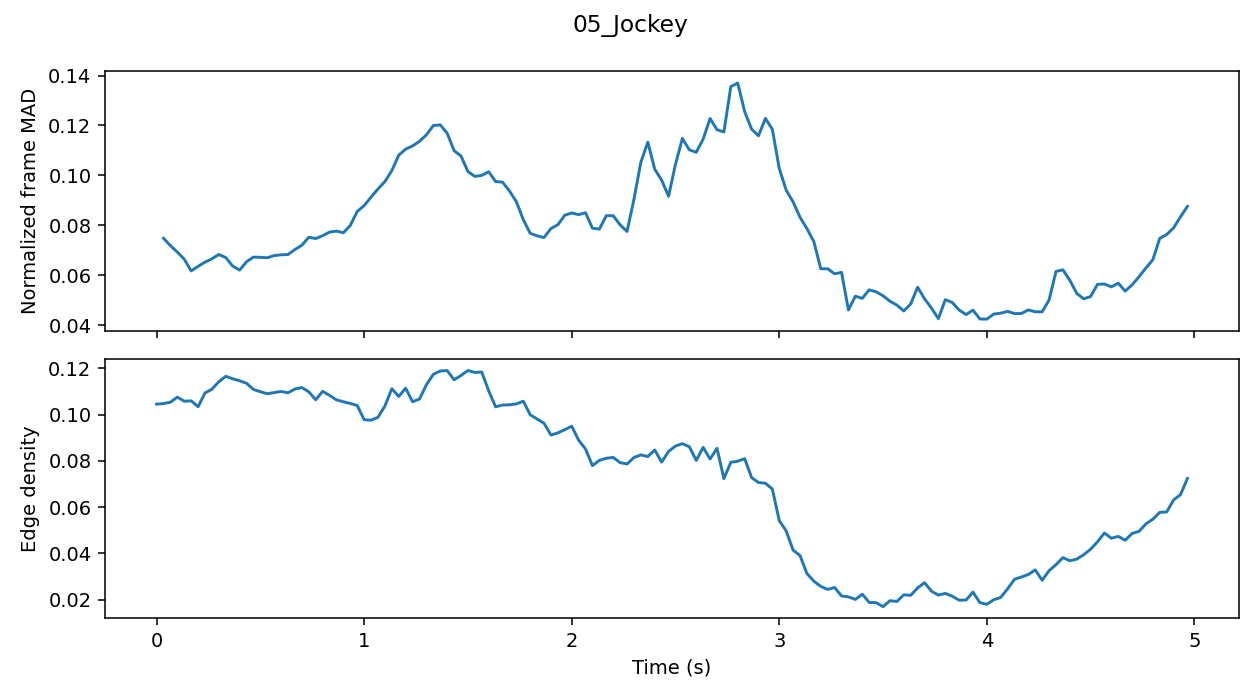
\includegraphics[width=.76\textwidth,height=.17\textheight,keepaspectratio]{experiments/full_exps/figures/05_Jockey_features.png}\\[-2pt]
\small Frame-level input features: normalized frame difference and Canny edge density.
\end{center}
\begin{center}
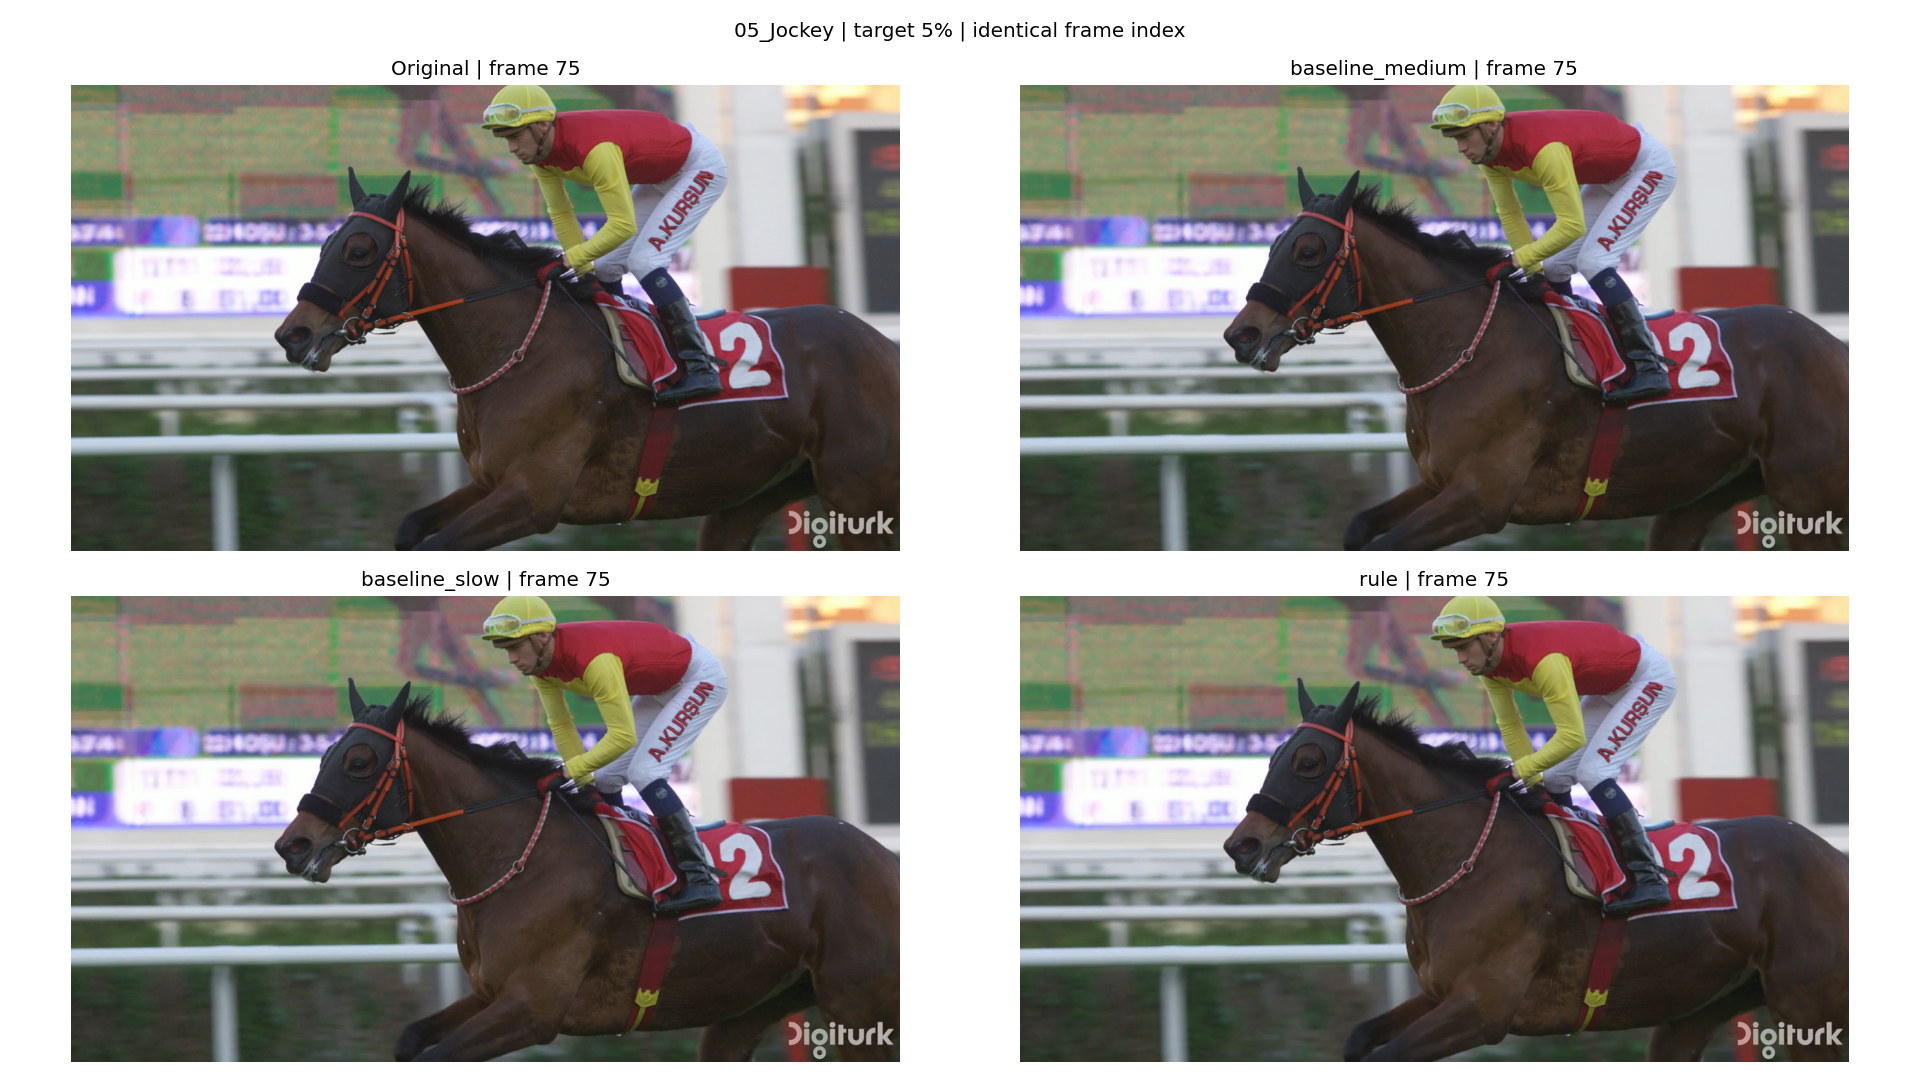
\includegraphics[width=.48\textwidth]{experiments/full_exps/figures/05_Jockey_0.05_comparison.png}\hfill
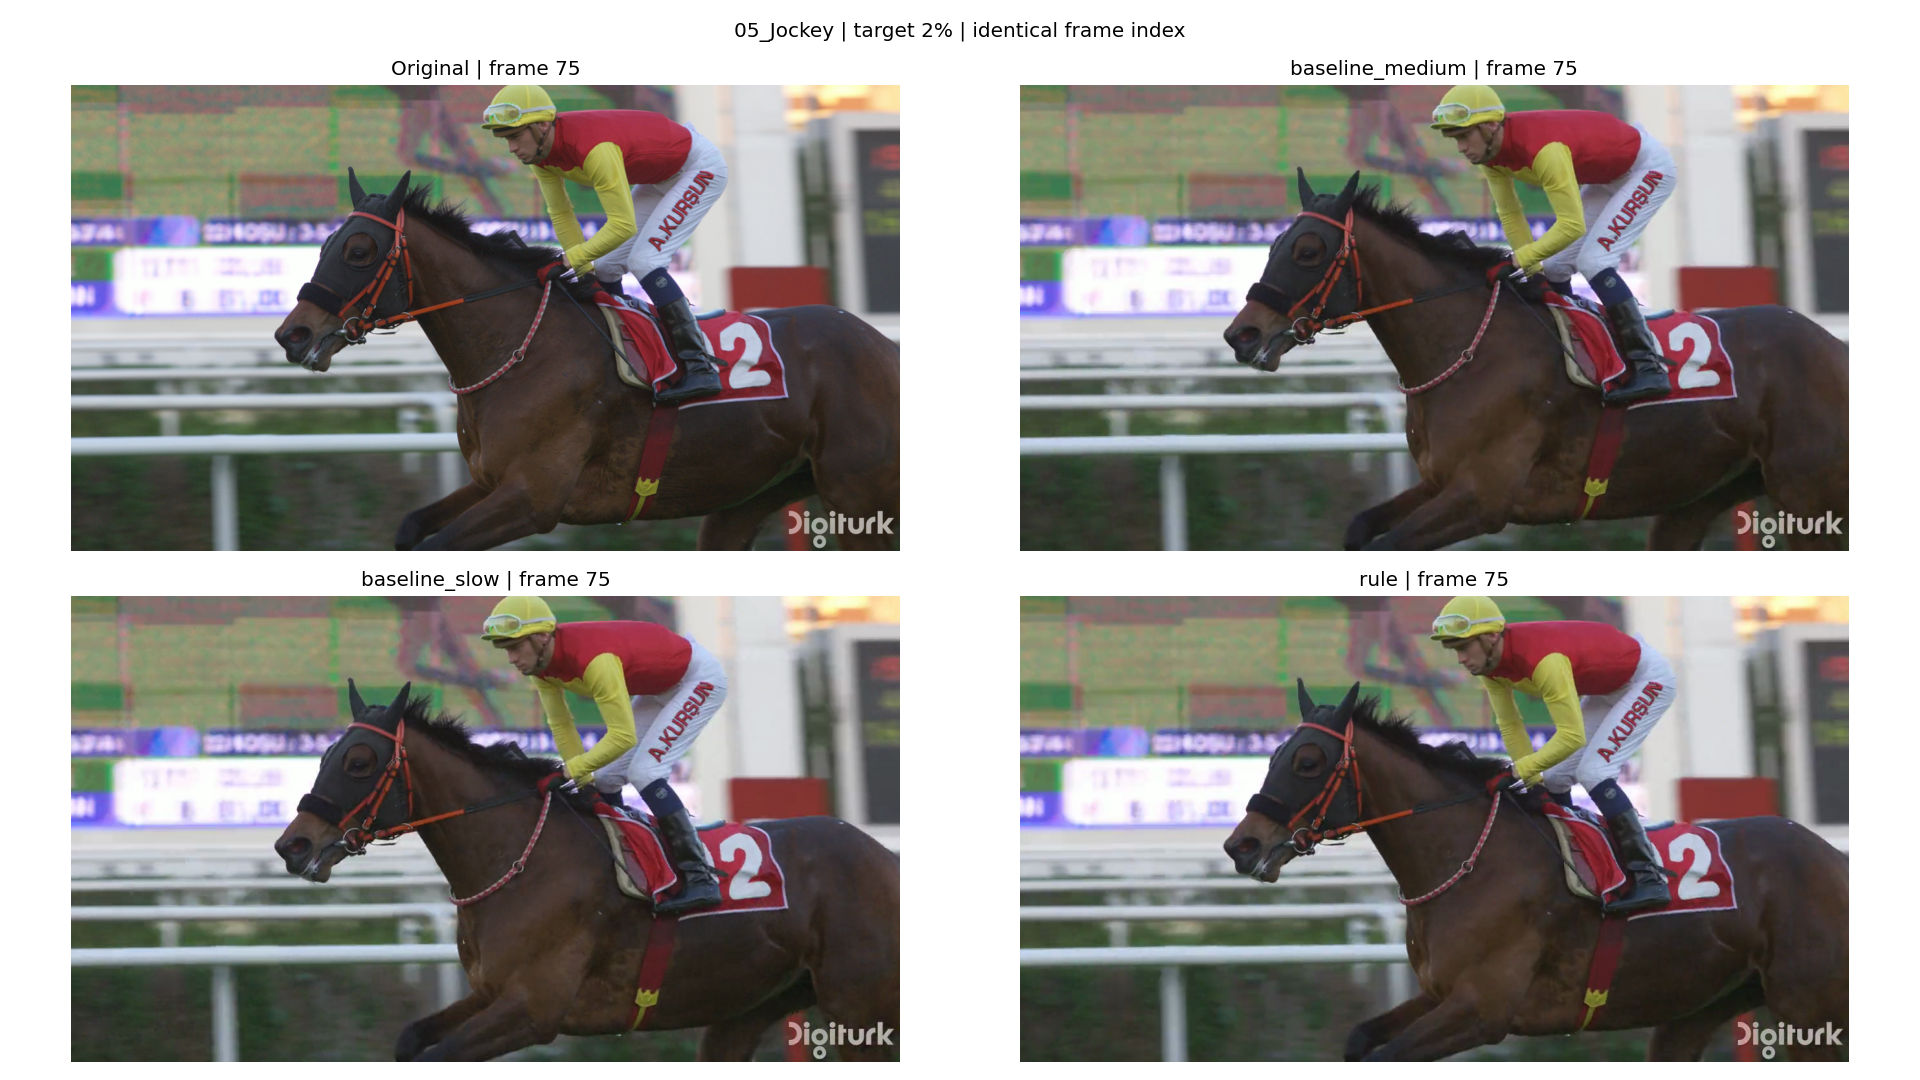
\includegraphics[width=.48\textwidth]{experiments/full_exps/figures/05_Jockey_0.02_comparison.png}\\[-2pt]
\small Source and decoded M/S/R outputs at 5\% (left) and 2\% (right).
\end{center}
\textbf{Measured decision and attempt log, 2\% target (1,422,014 bytes).} Values below are transcribed from the task and attempt records; rate is video target bitrate. Two passes count as one attempt.
\begin{center}\small\begin{tabular}{lrrrl}\toprule
Controller / attempt & AQ & Rate (bit/s) & MP4 bytes & Outcome\\\midrule
M / 1 & 1 & 2,229,717 & 1,427,075 & Oversized; retry\\
M / 2 & 1 & 2,177,373 & 1,389,090 & Accepted\\
R / 1 & 2 & 2,229,717 & 1,417,781 & Accepted\\\bottomrule\end{tabular}\end{center}
The rule's first output fits with 4,233 bytes remaining. M overshoots by 5,061 bytes and reduces the rate before its accepted second output. At 2\%, R achieves 39.891 dB / 0.986503 versus M's 39.813 dB / 0.986133; its final file is also larger. At 5\%, R obtains 43.189 dB / 0.994223 versus M's 43.168 dB / 0.994172. The 2\% comparison therefore combines AQ, accepted bitrate and attempt-count effects.
\clearpage
\subsection{06 ShakeNDry: AQ 1 with two-pass retry}
This 75-frame, 2.5-second UVG clip uses frame 37 for the panels. Motion mean is 0.014290 and edge mean is 0.183712. Since the edge mean exceeds 0.10101047, the rule selects medium/AQ 1. The rule and medium baseline produce byte-identical files at both budgets.
\begin{center}
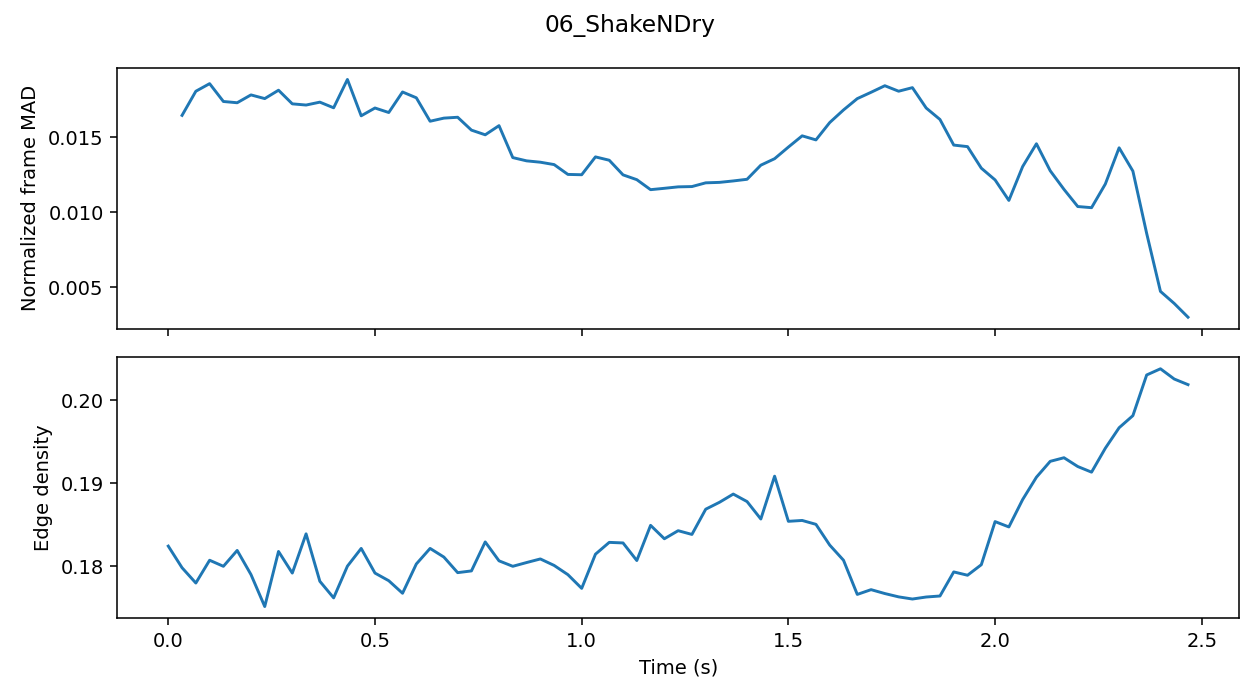
\includegraphics[width=.76\textwidth,height=.17\textheight,keepaspectratio]{experiments/full_exps/figures/06_ShakeNDry_features.png}\\[-2pt]
\small Input feature timeline; the horizontal axis spans 2.5 seconds.
\end{center}
\begin{center}
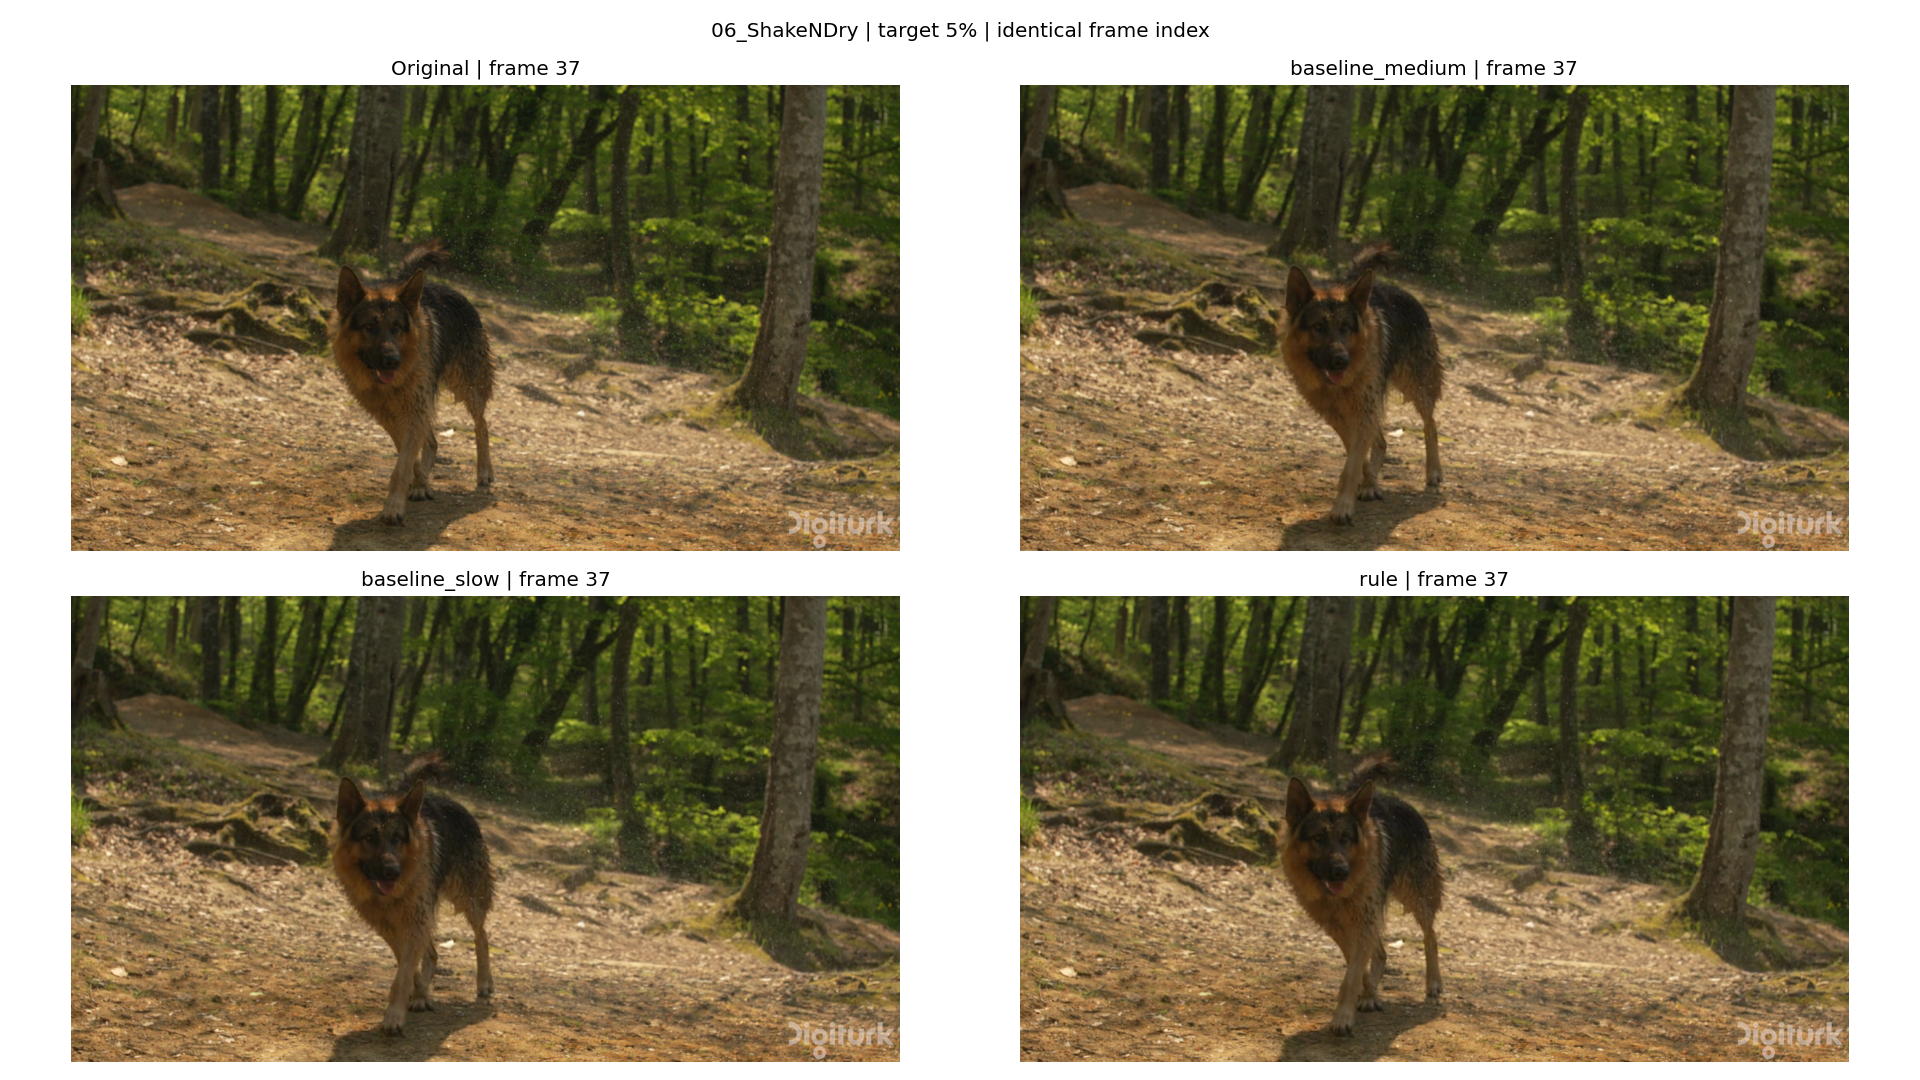
\includegraphics[width=.48\textwidth]{experiments/full_exps/figures/06_ShakeNDry_0.05_comparison.png}\hfill
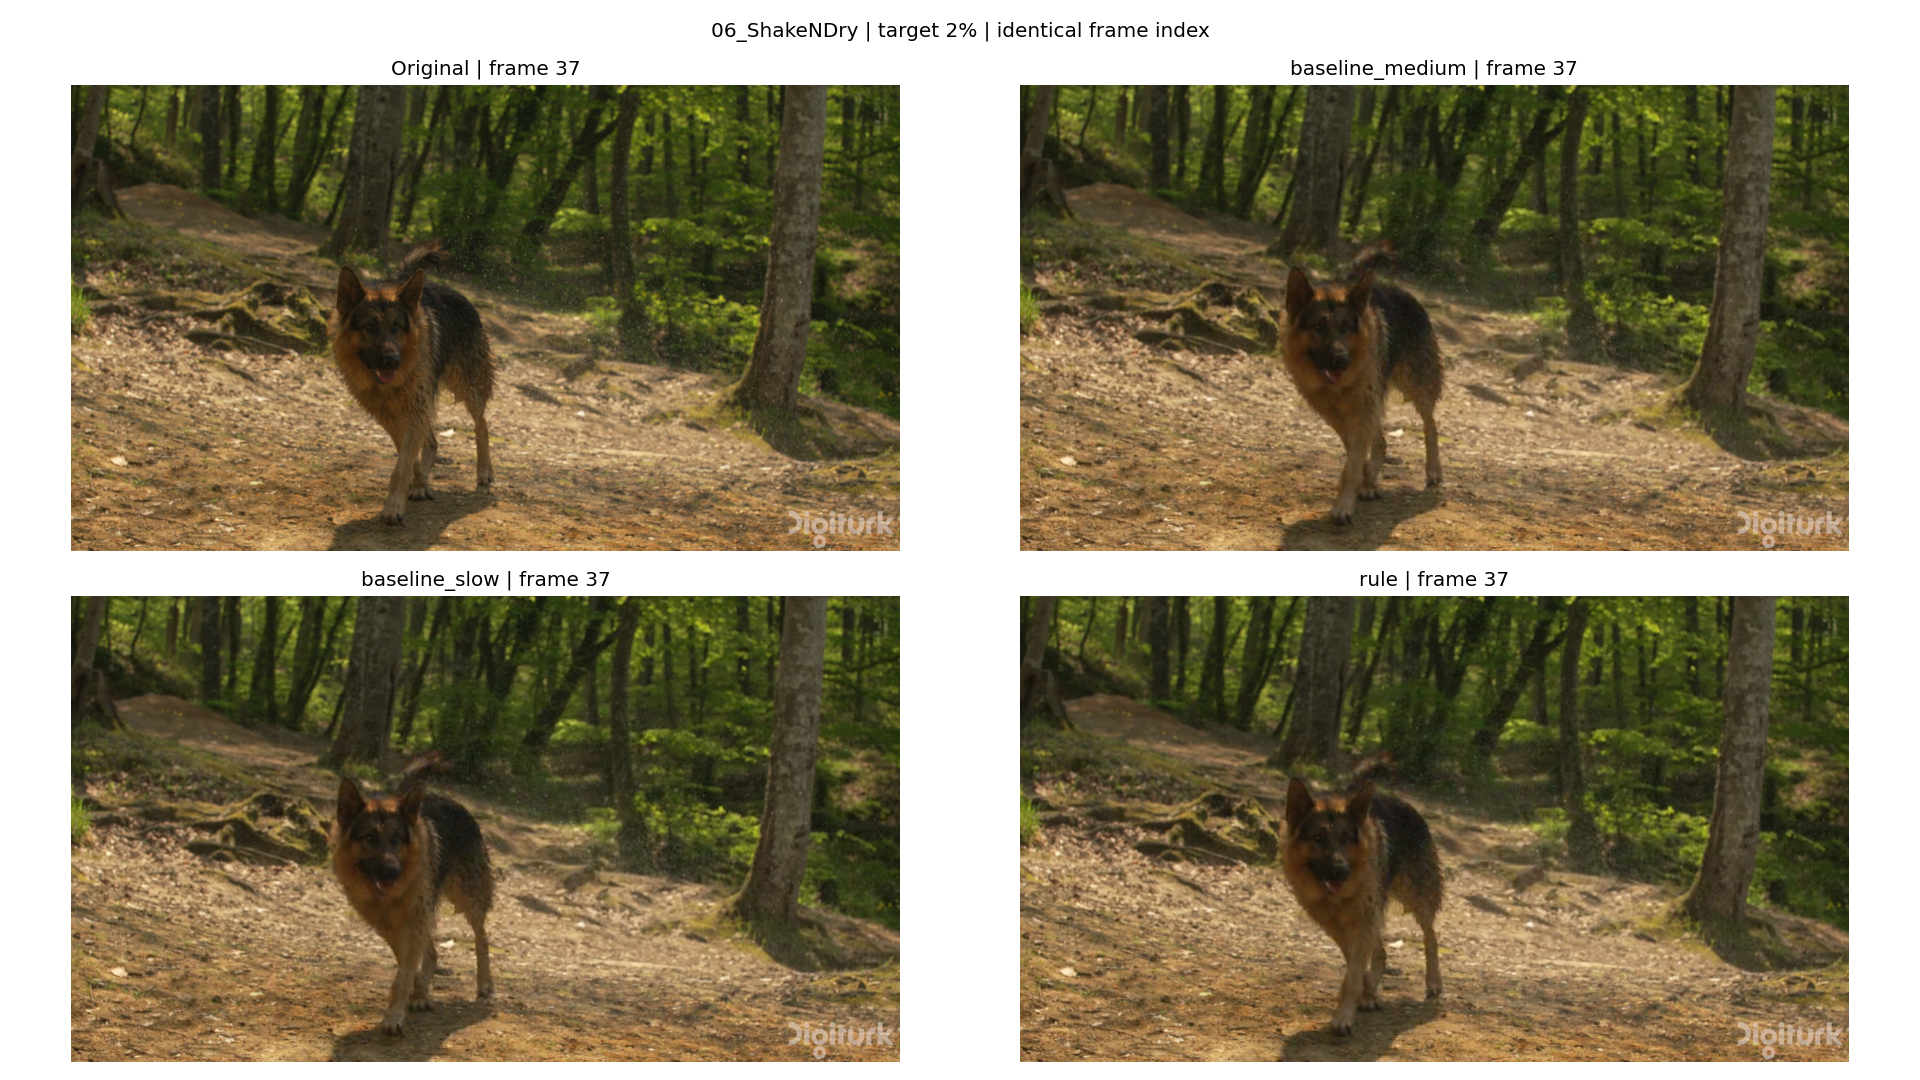
\includegraphics[width=.48\textwidth]{experiments/full_exps/figures/06_ShakeNDry_0.02_comparison.png}\\[-2pt]
\small Source and decoded M/S/R outputs at 5\% (left) and 2\% (right).
\end{center}
\textbf{Measured rule attempt log, 2\% target (823,665 bytes).}
\begin{center}\small\begin{tabular}{lrrrl}\toprule
Attempt & AQ & Rate (bit/s) & MP4 bytes & Outcome\\\midrule
1 & 1 & 2,583,013 & 921,911 & Oversized; retry\\
2 & 1 & 2,261,592 & 811,790 & Accepted\\\bottomrule\end{tabular}\end{center}
The first output exceeds the limit by 98,246 bytes. Proportional feedback lowers the video rate; the second output is 11,875 bytes below the limit. Both budgets need two attempts for all three groups. At 2\%, R and M score 36.817 dB / 0.982395, while S scores 36.735 dB / 0.982057. The unchanged R/M output is consistent with the same preset, AQ, bitrate path and source; it does not show a separate quality improvement from the rule.
\clearpage
\subsection{09 Parkrun: similar motion, different AQ}
This 150-frame, 5-second Xiph clip uses frame 75. Its mean motion is 0.078336, close to Jockey's 0.077560, but mean edge density is 0.258743, above the threshold. The frozen decision is medium/AQ 1. This pair illustrates which measured feature actually drives the decision.
\begin{center}
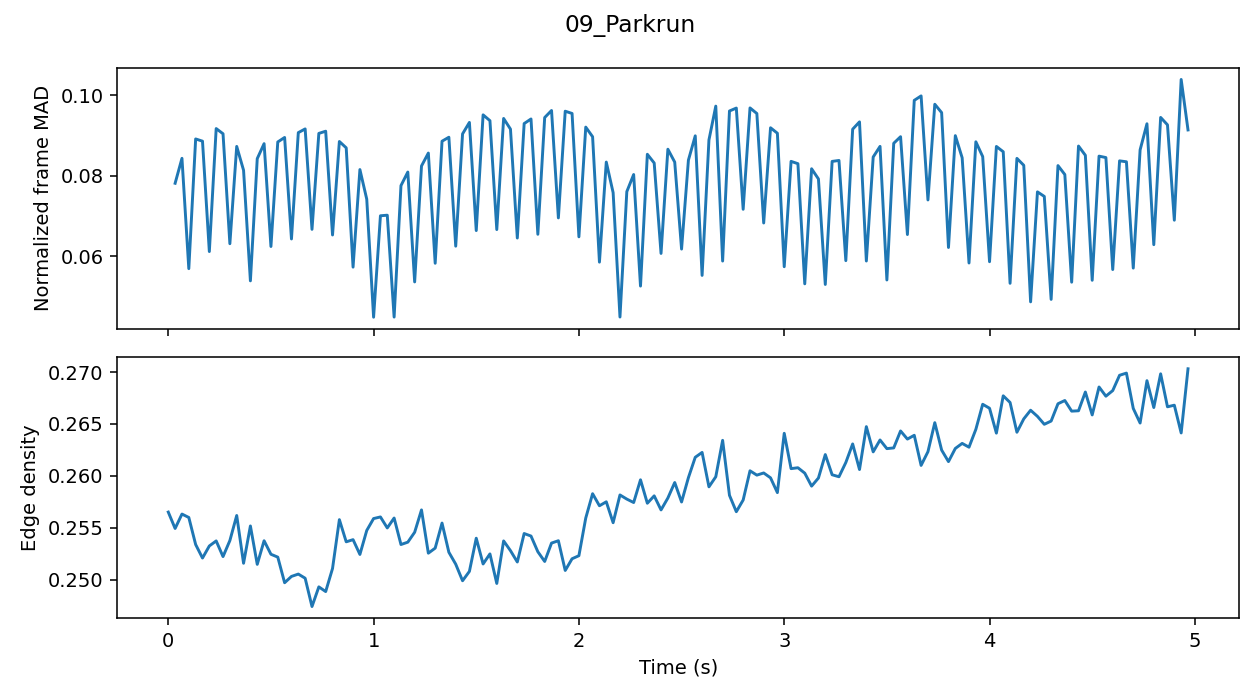
\includegraphics[width=.76\textwidth,height=.17\textheight,keepaspectratio]{experiments/full_exps/figures/09_Parkrun_features.png}\\[-2pt]
\small Input feature timeline: note the edge scale differs from the Jockey plot.
\end{center}
\begin{center}
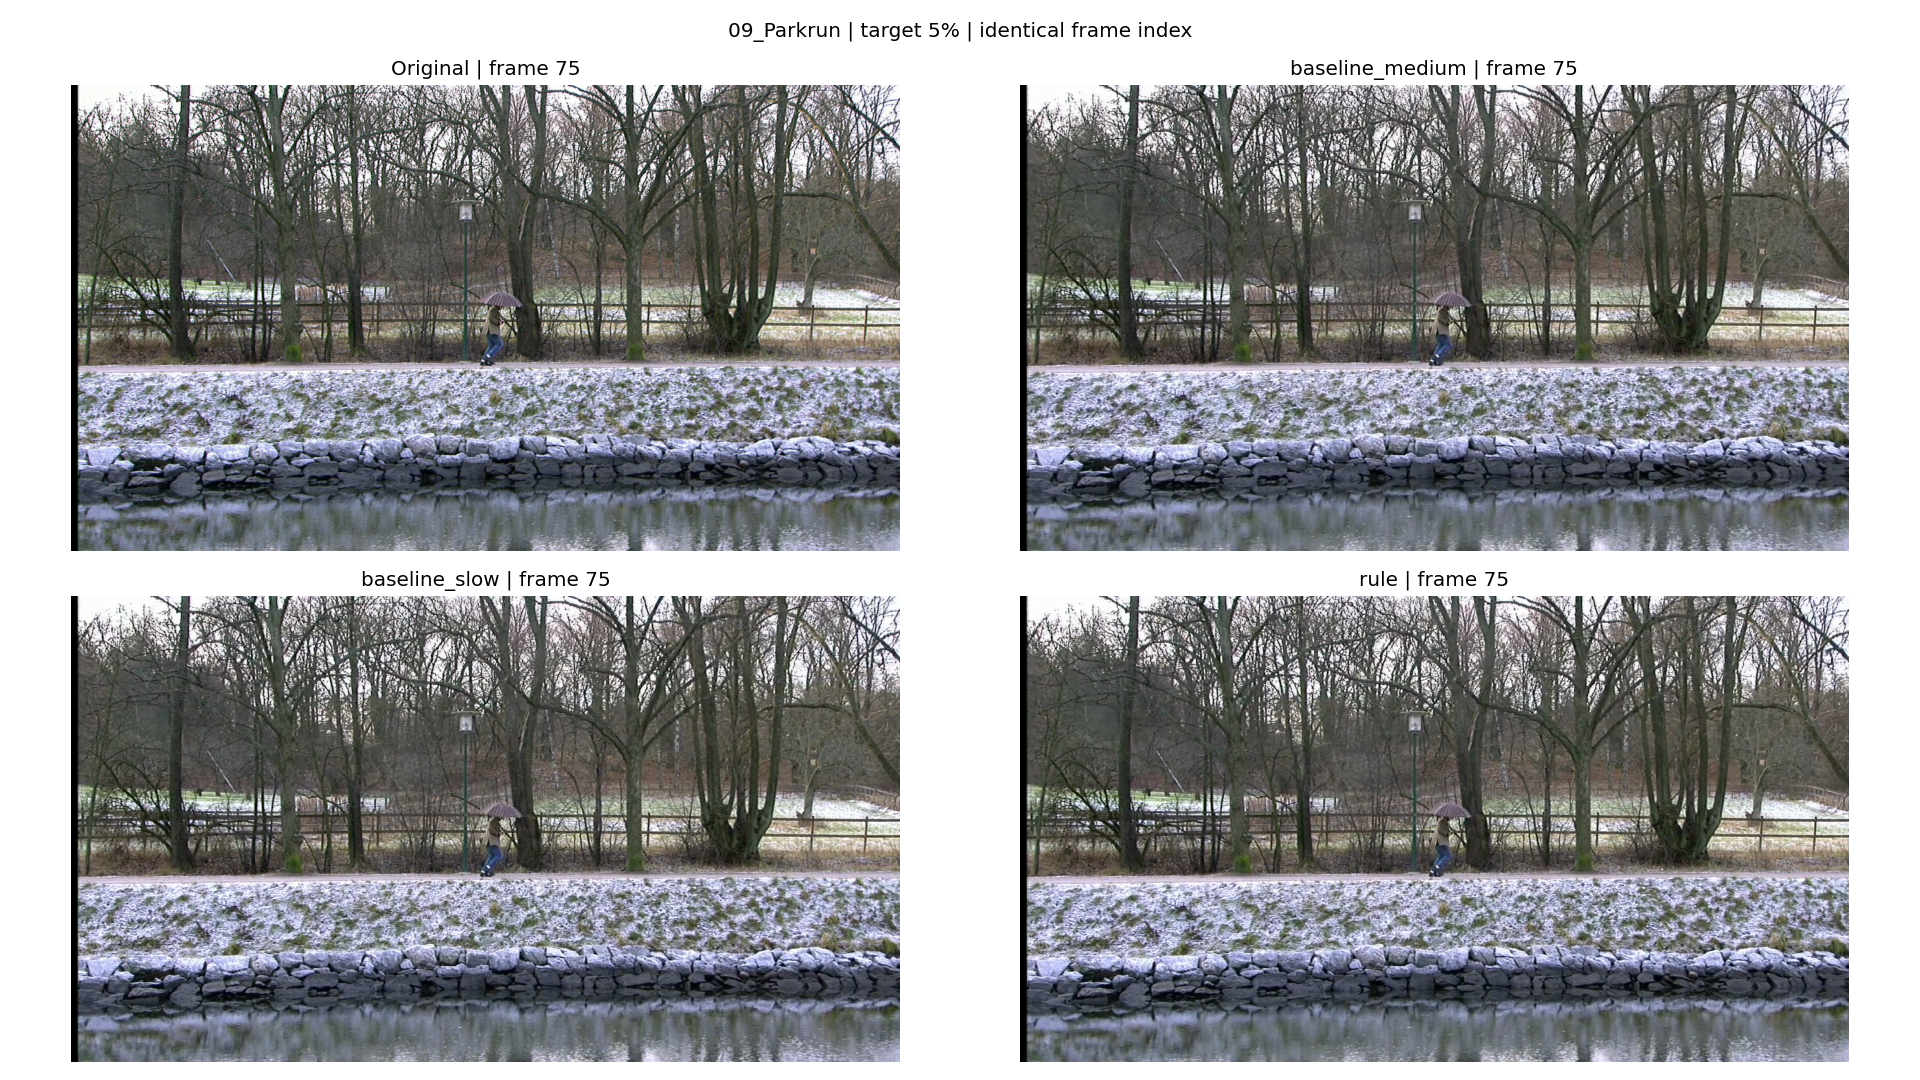
\includegraphics[width=.48\textwidth]{experiments/full_exps/figures/09_Parkrun_0.05_comparison.png}\hfill
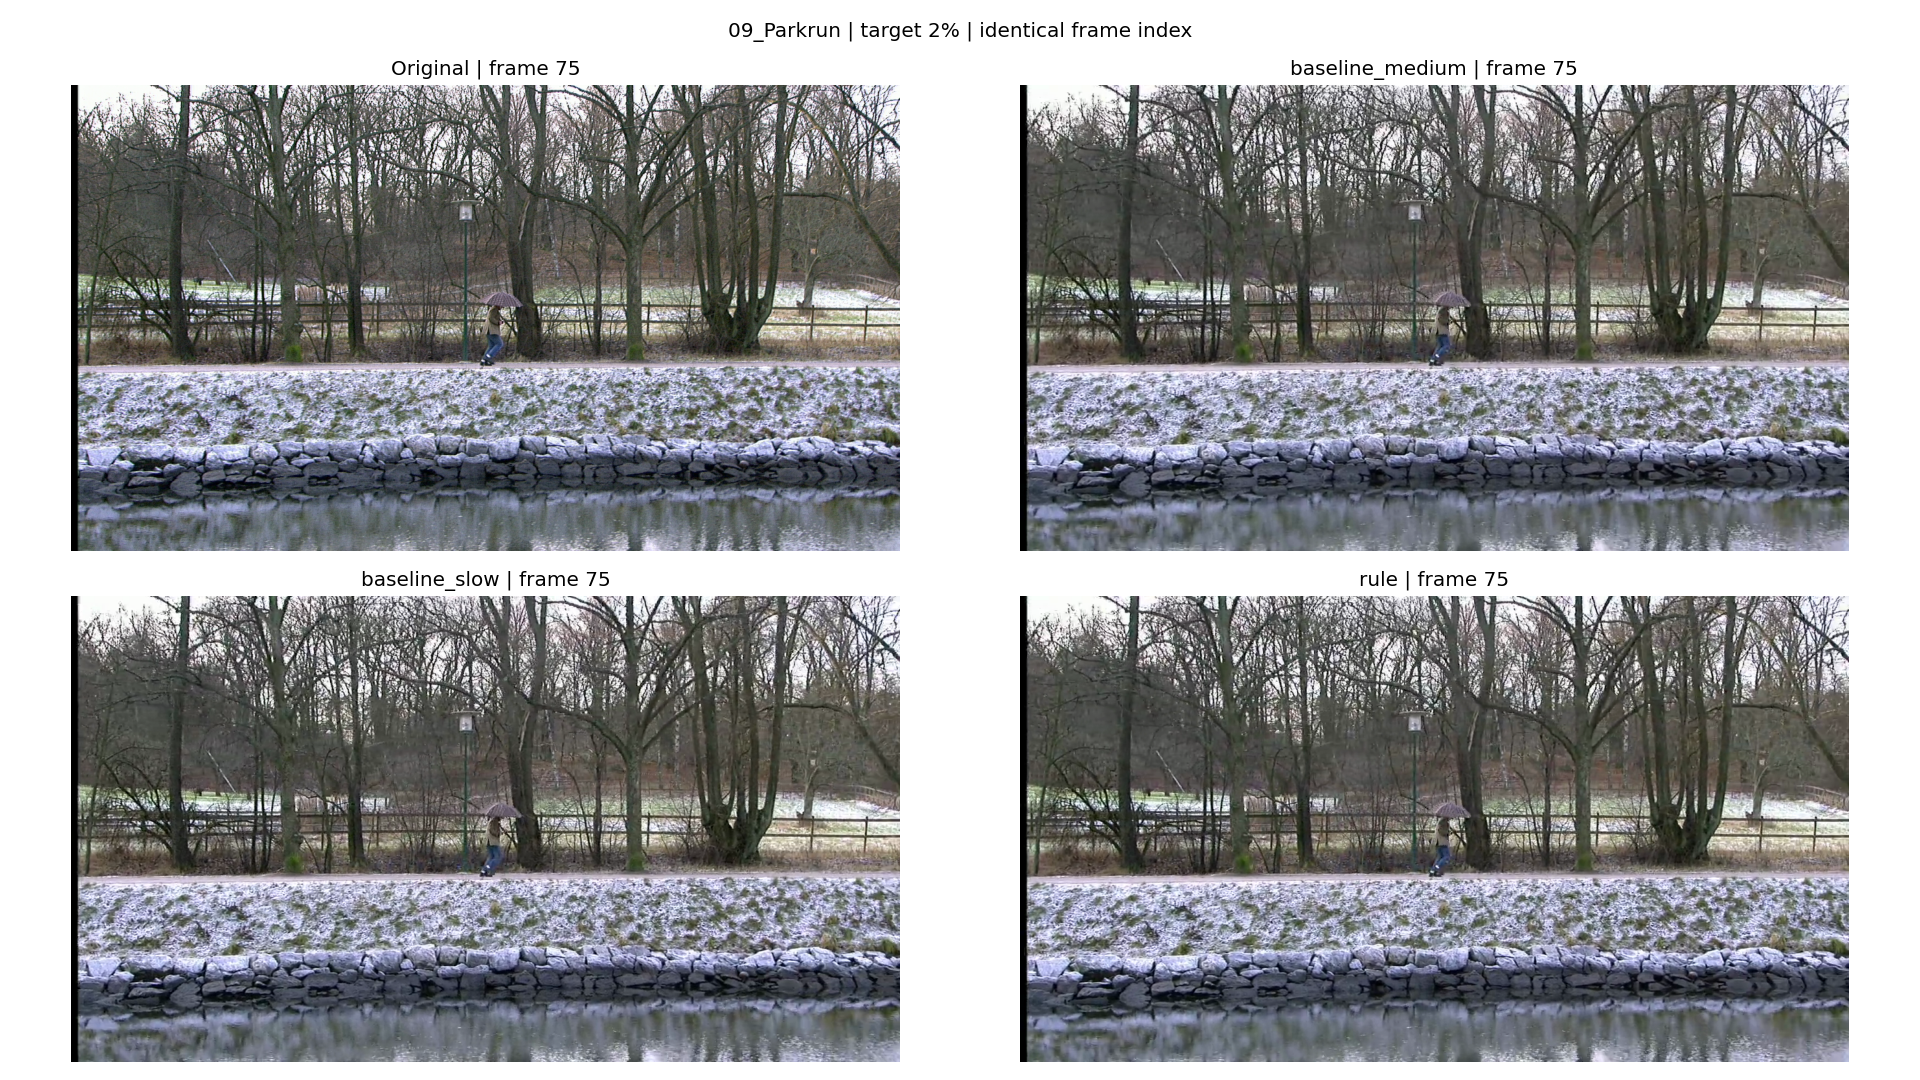
\includegraphics[width=.48\textwidth]{experiments/full_exps/figures/09_Parkrun_0.02_comparison.png}\\[-2pt]
\small Source and decoded M/S/R outputs at 5\% (left) and 2\% (right).
\end{center}
\textbf{Measured rule decisions and accepted outputs.}
\begin{center}\small\begin{tabular}{lrrrrr}\toprule
Budget & AQ & Rate (bit/s) & Limit (bytes) & MP4 bytes & PSNR (dB)\\\midrule
5\% & 1 & 9,092,068 & 5,798,513 & 5,592,701 & 29.932\\
2\% & 1 & 3,636,827 & 2,319,405 & 2,241,278 & 26.606\\\bottomrule\end{tabular}\end{center}
Both outputs pass on the first attempt and are byte-identical to M. Rule MS-SSIM falls from 0.982604 at 5\% to 0.962347 at 2\%, a decrease of 0.020257. This is a within-video budget comparison; it does not isolate a preset or AQ effect.

\textbf{Separate Ark cases and limitations.} One request each for clips 10, 11 and 12 at 2\% returned a response but failed unique-JSON validation, and no encoding occurred. An earlier independent Jockey 2\% Ark attempt successfully selected medium/AQ 2 and matched the pilot rule output byte-for-byte; three earlier pilot requests failed. These observations are separate from the 72 local tasks and do not establish model superiority. The evaluation contains short silent clips, no subjective viewing study and no repeated timing trials. The source frames derive from UVG and Xiph collections; plots are produced from measured input frames. The measured environment used macOS 26.2 arm64, FFmpeg 9.1, libx264 core 165 revision 3222 and two threads.
\begin{center}
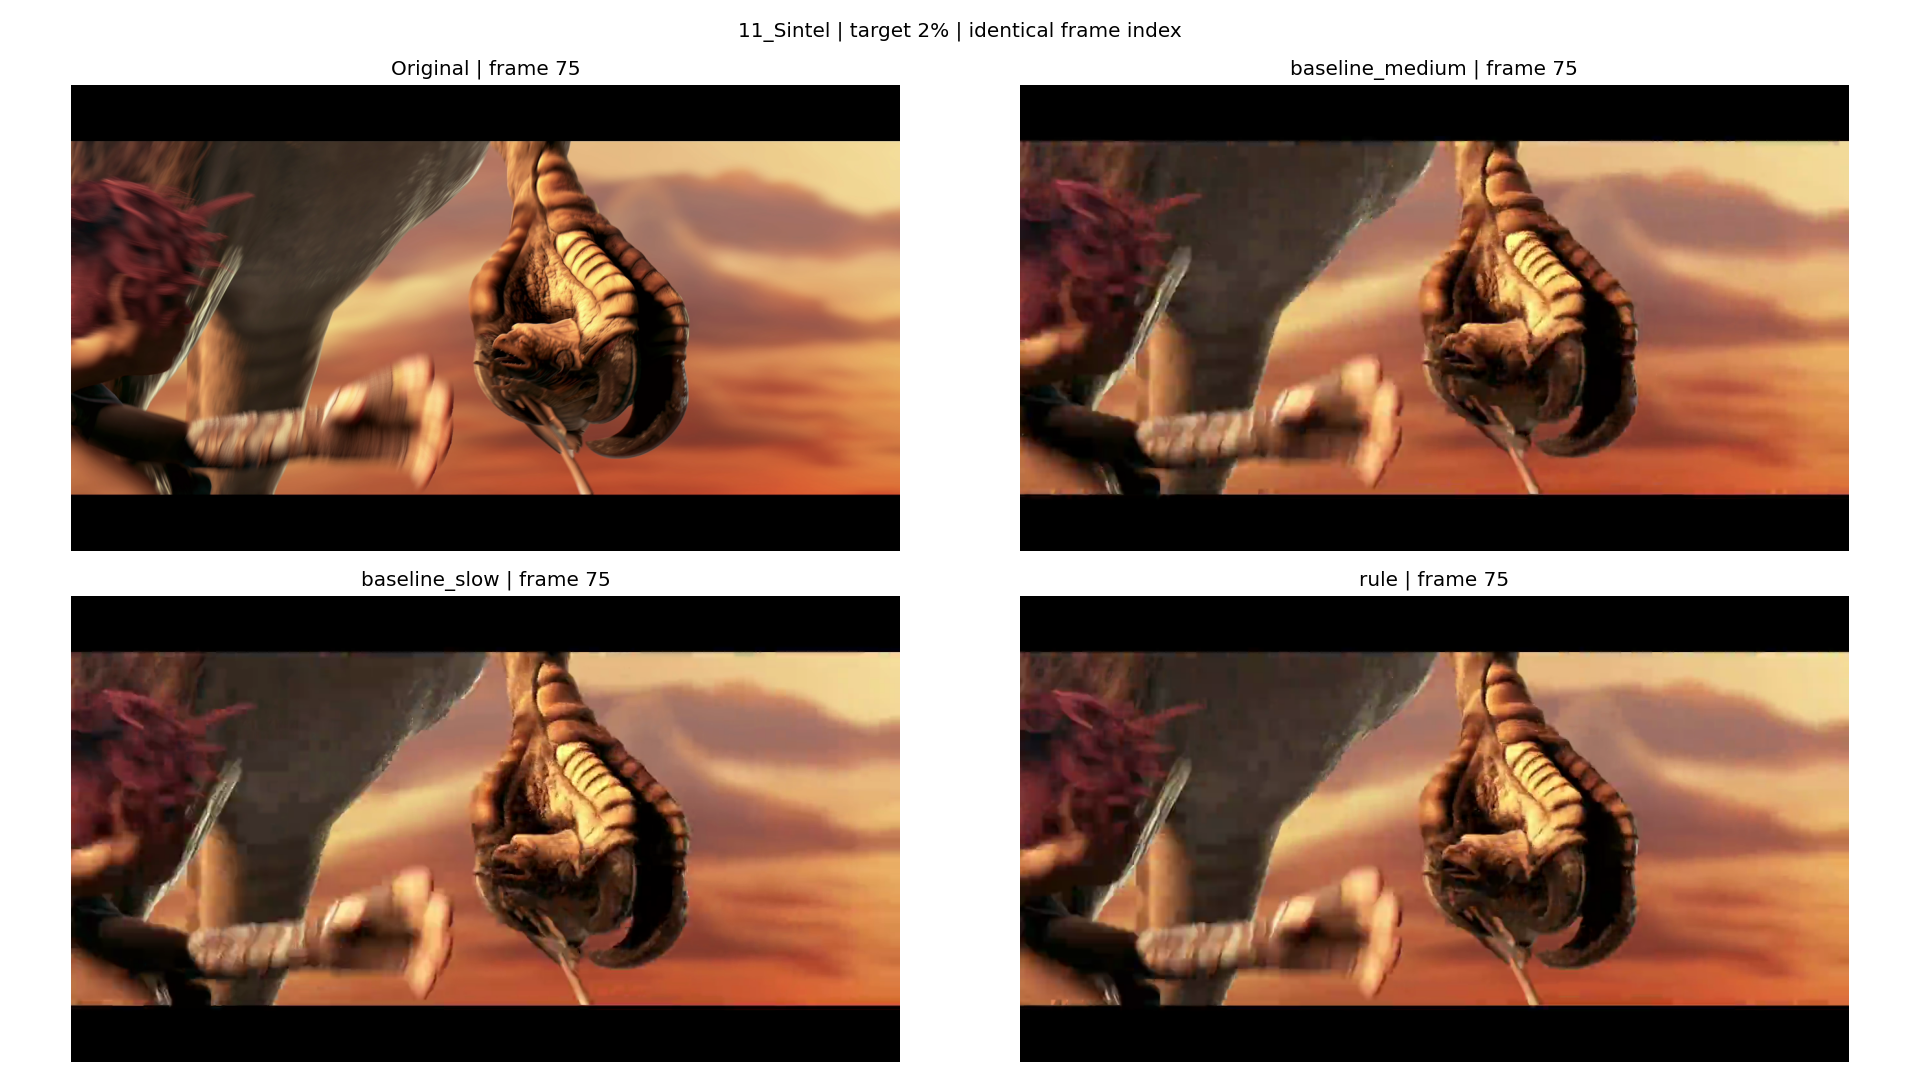
\includegraphics[width=.44\textwidth,height=.145\textheight,keepaspectratio]{experiments/full_exps/figures/11_Sintel_0.02_comparison.png}\hfill
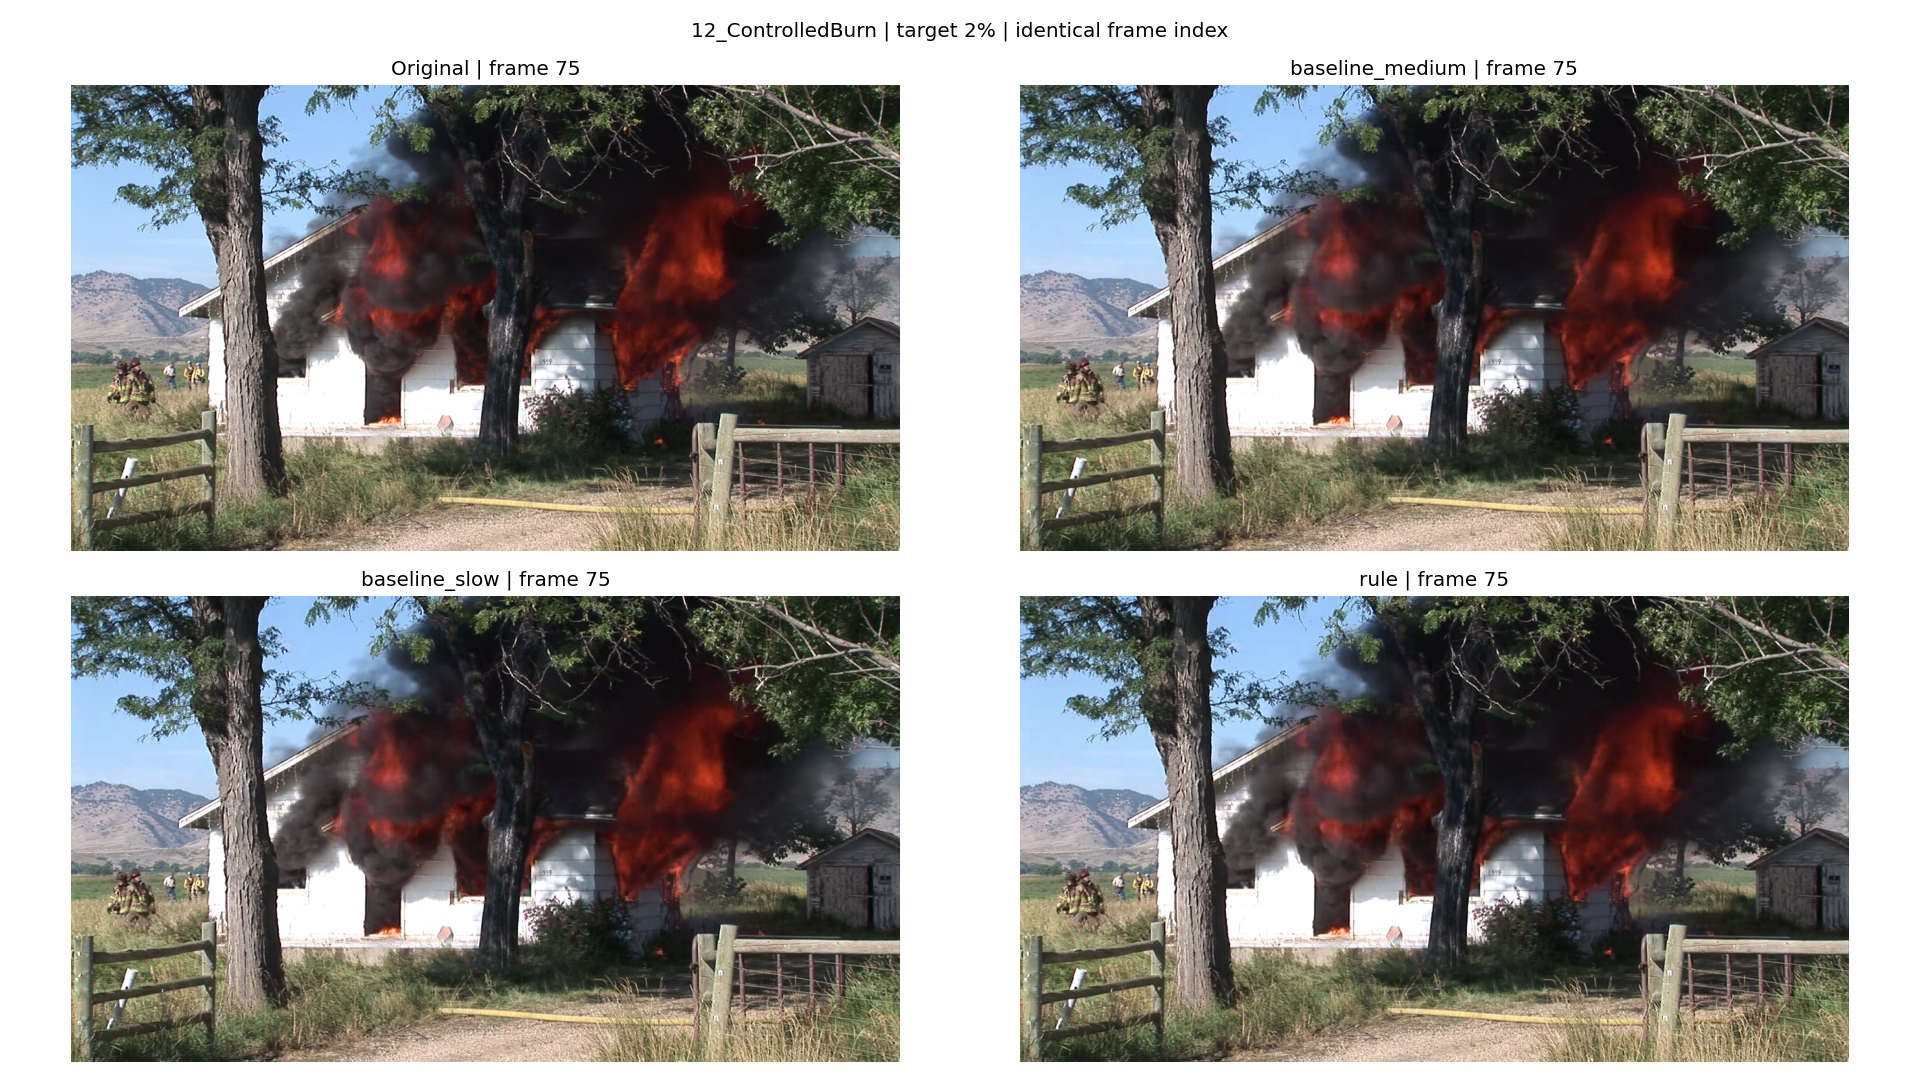
\includegraphics[width=.44\textwidth,height=.145\textheight,keepaspectratio]{experiments/full_exps/figures/12_ControlledBurn_0.02_comparison.png}\\[-2pt]
\small Additional 2\% comparisons: Sintel (left), ControlledBurn (right), frame 75.
\end{center}
Sintel at 2\%: rule AQ 2 achieves 38.094 dB versus medium AQ 1 at 37.619 dB; both require two attempts. ControlledBurn uses AQ 1 and its rule and medium outputs are byte-identical.
\end{document}
